\documentclass[t,10pt,hyperref={
  %pdfpagemode=FullScreen,
  pdftitle = {gearshifft},
  pdfsubject = {gearshifft},
  %linktocpage=true,
  pdfborder={0 0 0},
  colorlinks=true,
  urlcolor=red,
  citecolor=red,
  linkcolor=red,
  pdfauthor={Peter Steinbach, Matthias Werner}
  }
]{beamer}
\usetheme{custom}
\def\resetbeamertemplate{\setbeamertemplate{background canvas}{ }}
\let\Tiny=\tiny
%\usepackage{lmodern}
\usepackage{tikz}
\usetikzlibrary{matrix}
\usetikzlibrary{calc}
\usetikzlibrary{positioning}
% \usepackage[utf8]{inputenc}
% \usepackage[T1]{fontenc}
\usepackage[utf8]{inputenc}
\usepackage[T1]{fontenc}
\usepackage{csquotes}

\usepackage{amsmath,amstext,amsthm,array,booktabs}
\usepackage{caption}
\usepackage{xcolor}
\usepackage{graphicx}
\usepackage{colortbl}
\usepackage{listings}
\usepackage{dirtree}

\usepackage[%per=slash,
%            decimalsymbol=comma,
            locale=US,
            ]{siunitx}

%%%%%%%%%%
\providecommand\thispdfpagelabel[1]{}

% \mode<presentation>{%
% \setbeameroption{show notes}
% }

\newcolumntype{M}{>{$\displaystyle}l<{$\vspace{1ex}}}
\title{gearshifft -- The FFT Benchmark Suite for Heterogeneous Platforms}
\author{
  \parbox{0.44\textwidth}{%\centering %
    Peter Steinbach\\[.5em]
    {\footnotesize{Max Planck Institute of Molecular Cell Biology and Genetics}}\\
    {\small{01307 Dresden, Germany\\
    \url{steinbac@mpi-cbg.de}}}}
\hfill
\parbox{0.47\textwidth}{
  Matthias Werner\\[.5em]
{\footnotesize{Center for Information Services and High Performance Computing}}\\
{\small{TU Dresden, Germany\\
\url{Matthias.Werner1@tu-dresden.de}}}}
}

\date{2017/06/20}

%%%%%%%%%%%%%%%%%%%%%%%%

\newcommand\mlhead[2]{%
  \multicolumn{1}{l}{\parbox{#1}{\centering #2}}
}
%%%%%%%%%%%%%%%%%%%%%%%%%%%%
\definecolor{arccl}{rgb}{0.45,0.45,0.45}
\newcommand{\mgraymidrule}{\arrayrulecolor{arccl}\midrule\arrayrulecolor{black}}
%%%%%%%%%%%%%%%%%%%%%%%%%%%%%%%%%%%%%%%%%%%%%%%%%%%%%%%%%%%%%%%%%%%%%%%%




\newcommand{\gearshifft}{\texttt{gearshifft}}
\newcommand{\fftw}{\texttt{fftw}}
\newcommand{\cufft}{\texttt{cuFFT}}
\newcommand{\clfft}{\texttt{clFFT}}
\newcommand{\nvidia}{Nvidia}
\newcommand{\mc}[1]{\lstinline!#1!}
\newcommand{\iu}{{\mathrm{i}\mkern1mu}}

%%
\begin{document}
\frame[plain]{\titlepage}

% \begin{frame}
% 	\frametitle{Table of Contents}
% 	\tableofcontents%[pausesections]
% \end{frame}

\begin{frame}{Introduction}
  % fft use cases
  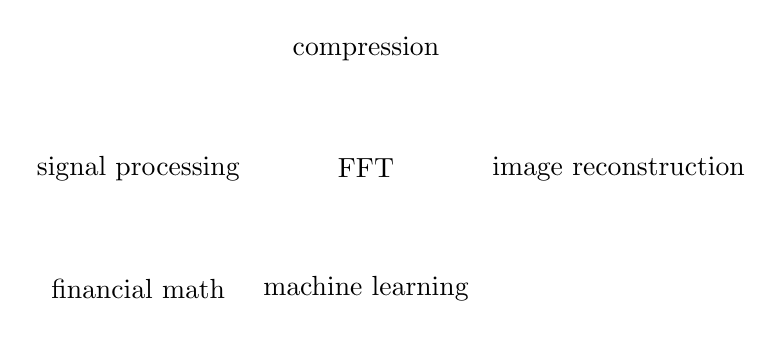
\begin{tikzpicture}%[every node./style={draw={rectangle}}]
    \node (fft) {FFT};
    \node[left=1cm of fft] (sign) {signal processing};
    \node[right=1cm of fft] {image reconstruction};
    \node[above=1cm of fft] {compression};
    \node[below=1cm of fft] {machine learning};
    \node[below=1cm of sign] {financial math};
  \end{tikzpicture}
    
\end{frame}

\begin{frame}{FFT}

  \begin{equation}
    \label{eq:dft}
    X[k] = \sum_{j=0}^{n-1} x[j]\cdot\exp\left(\frac{-2\pi \iu jk}{n}\right),\quad x,X\in\mathbb{C}^n
  \end{equation}
  
  \begin{itemize}
  \item fast implementation of the discrete Fourier transform (DFT) \eqref{eq:dft}
  \item forward transform: time domain $\Rightarrow$ frequency domain
  \item by factorization of $n$ and recursive decomposition smaller DFTs are computed
  \item $\mathcal{O}(n\log n)$
  \item Cooley-Tukey: Radix-2 DFTs
  \item Stockham's formulations avoids incoherent memory access
  \item Bluestein's algorithm allows arbitrary and mixed radices
  \item FFT libraries fftw, clFFT, cuFFT, hcFFT, \ldots 
  \end{itemize}

\end{frame}

\begin{frame}{Hardware}
  \begin{itemize}
  \item 
  \end{itemize}
\end{frame}

\definecolor{mc1}{rgb}{0.0, 1.0, 1.0}
\definecolor{mc2}{rgb}{0.0, 1.0, 0.0}
\definecolor{mc3}{rgb}{0.0, 1.0, 0.65}
\begin{frame}{Fileserver}
\begin{minipage}{0.4\textwidth}
%  \centering
\dirtree{%
.1 \color{mc1}{.}.
.1 \color{mc2}{Alle\_(Institut)}.
.1 \color{mc1}{Baustoffe}.
% .2 Alle\_(Baustoffe).
.1 \color{mc1}{Glas}.
.2 \color{mc3}{Alle\_(Glas)}.
.3 \color{mc3}{Anleitungen}.
.3 \color{mc3}{Eingaenge}.
.3 \color{mc3}{Marketing}.
.2 \color{yellow}{Alter\_Fileserver}.
% .3 Eingaenge.
% .3 glas.
% .3 Publikationen.
% .3 Saftware.
% .3 Vorlagen.
.2 \color{mc1}{Intern}.
.2 \color{mc1}{PG\_Ancorro}.
.2 \color{mc1}{PG\_B230}.
.2 \color{mc1}{PG\_CompGlass}.
.2 \color{mc1}{PG\_CoReCon}.
.2 \color{mc1}{PG\_Email}.
.2 \color{mc1}{PG\_Fugenmasse}.
.2 \color{mc1}{PG\_Schunk}.
.1 \color{mc1}{Keramik}.
% .2 Alle\_(Keramik).
}

\end{minipage}
\hfill
\begin{minipage}{0.5\textwidth}
%  \centering
 Zugriffsmodi:\\
 {\color{mc2}{Lesen und Schreiben}} (IKGB)\\
 {\color{mc3}{Lesen und Schreiben}} (Glas)\\
 {\color{yellow}{Lesen}} (Glas)\\
 {\color{mc1}{Geschützt}}
\end{minipage}

\end{frame}


\end{document}

%%% Local Variables:
%%% mode: latex
%%% TeX-master: t
%%% End:
